\documentclass[11pt,a4paper]{article}
\usepackage[utf8]{inputenc}
\usepackage[T1]{fontenc}
\usepackage{amsfonts}
\usepackage[french]{babel}
\frenchbsetup{StandardLists=true} % à inclure si on utilise \usepackage[francais]{babel}
\usepackage{enumitem}
\usepackage{amssymb}
\usepackage{amsmath}
\usepackage[left=2cm,right=2cm,top=2cm,bottom=2cm]{geometry}
\usepackage[dvipsnames]{xcolor}

\usepackage[T1]{fontenc}
\usepackage{fouriernc}
\usepackage{graphicx}

\usepackage{setspace}
\singlespacing

\usepackage{colortbl}
\usepackage{tikz}
\usepackage{tikz-osci}
\AtBeginDocument{\shorthandoff{;}}

\usepackage{amssymb}
\usepackage{multicol}
\usepackage{caption}
\usepackage{fancyhdr}
\pagestyle{fancy}
\renewcommand\headrulewidth{1pt}
\fancyhead[L]{Lycée Denis Diderot }
\fancyhead[L]{Lycée Denis Diderot }
\fancyhead[R]{Classe de 1 Bac Pro }
\setcounter{page}{6}\fancyfoot[C]{page \thepage}
\fancyfoot[R]{Année 2024-2025}
\fancyfoot[L]{Alexis RUIZ}
\usepackage{multirow,tabularx,booktabs}
\newcommand{\cadreblanc}[1]{%
\medskip\framebox[\linewidth][c]{%
\rule{0mm}{#1mm}}\par
\medskip}

\usepackage{awesomebox}
\setlength{\aweboxvskip}{0mm}
\usepackage{pifont}
\usepackage{chemmacros}
\chemsetup{modules=all}
%\setlength{\columnseprule}{.25mm}

\renewcommand{\arraystretch}{3.5}
\newcolumntype{C}[1]{>{\centering\arraybackslash }p{#1}}

\newcommand*\acocher{\quitvmode{\fboxsep0pt \fboxrule0.8pt \fbox{\vrule height1.8ex depth.1ex width0pt \vrule height0pt depth0pt width1.9ex }}}

\newcommand{\code}{\awesomebox[black]{2pt}{

\includegraphics[scale=0.15]{../Chapitre 1 - Energie et puissance électrique/images/frame.png}
}{black}}

\newcommand{\moteur}{\awesomebox[black]{2pt}{

\includegraphics[scale=1]{images/moteur.jpg} 
}{black}}

\newcommand{\defconclusion}{\awesomebox[black]{2pt}{\rotatebox{90}{\Large{\textbf{Conclusion}}}}{black}}


  \newenvironment{itemize*}%  % listes compactes
    {\begin{itemize}%
      \setlength{\itemsep}{0pt}%
      \setlength{\parskip}{0pt}}%
    {\end{itemize}}


\frenchbsetup{StandardLists=true}


\frenchbsetup{StandardLists=true}
\newlist{fleche}{itemize}{1}
\setlist[fleche]{label=\ding{220},font=\color{orange}}



\begin{document}


\begin{center}
 \LARGE{Exercices } \\[3mm]
\end{center}



\normalsize

\hrule\
\\[0,5cm]



\fbox{\textbf{Exercice 1 }} ~QCM : Parmi les trois propositions, choisissez la bonne réponse. 

\begin{center}



    \begin{tabular}{|C{0.5cm} p{5.5cm}|C{3cm}|C{3cm}|C{3cm}|}
         \hline
       \ding{202} &Les courbes ci-dessous 
       & $\Box $ ~~sont en phase & $\Box $ ~~sont déphasées & $\Box $ ~~ont le même déphasage\\
       
         &
       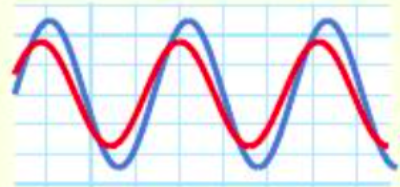
\includegraphics[scale=0.2]{images/qcm1.png}
       & &  & \\

       \hline
       
      \ding{203}&$\Delta t$ représente & $\Box $ ~~le décalage temporel entre $u(t)$ et $i(t)$ & $\Box $ ~~le facteur de puissance  & $\Box $~~le déphasage entre $u(t)$ et $i(t)$ \\
         \hline
       
      \ding{204}&$\varphi$ représente & $\Box $ ~~le décalage temporel entre $u(t)$ et $i(t)$ & $\Box $ ~~le facteur de puissance  & $\Box $~~le déphasage entre $u(t)$ et $i(t)$ \\
      
         \hline
         
         \ding{205} &Pour un récepteur électrique $\cos \varphi$ est ...& $\Box $ ~~ le déphasage & $\Box $ toujours supérieur à 1& $\Box $ ~~ le facteur de puissance\\
         
         \hline
         
         %\ding{206}& Pour un récepteur ohmique (R)   &$\Box $ ~~ $\varphi =0$& $\Box $ $\varphi=\dfrac{\pi}{2}$& $\Box $ ~~ $\varphi=-\dfrac{\pi}{2}$\\
         %\hline
         \ding{206}&Pour mesurer la puissance consommée par un moteur, modélisé par une bobine et une résistance en série, il faut mesurer la tension $U$ entre  & $\Box $ ~~ M et N& $\Box $ M et P & $\Box $ ~~  N et P \\
         
         & 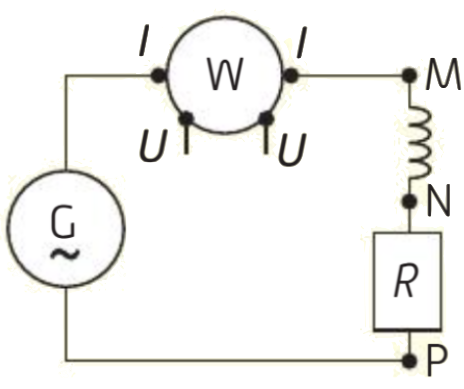
\includegraphics[scale=0.2]{images/qcm22.png} & & & \\

         \hline

         \ding{207} &L 'intensité traversant un moteur tel que $\cos \varphi =0,92$ consommant P=2 kW, sous une tension U~=~230~V est &$\Box$ ~~ i = 0,0945 A& $\Box$ i = 9,45 A &$\Box$ ~~ i = 14,35 A\\
         \hline
     

         
        
    \end{tabular}
\end{center}

\newpage

\fbox{\textbf{Exercice 2 }} : En utilisant la formule $P=U \times I \times \cos \varphi$, compléter le tableau ci-dessous : \\[5mm]

\begin{center}

    \renewcommand{\arraystretch}{3}


    \begin{tabular}{|p{3cm}|C{3cm}|C{3cm}|C{3cm}|}
         \hline
      $P (kW)$ &  $U(V)$ & $I (A)$ & $\cos \varphi$\\
         \hline 
         1,4 &  230  & 6,5& \\
         \hline
        & 230 & 9,7  & 0,86 \\
         \hline 
         4,5& 230 & 20,5  & \\
         \hline
         

    \end{tabular}\end{center}

    \vfill 


\fbox{\textbf{Exercice 3 }}\\[5mm]

\noindent%
\begin{minipage}{.36\textwidth}%
L'oscillogramme ci-contre représente deux signaux électriques sinusoïdaux ayant la même période $T$. \\
\vspace{-3mm}
\begin{enumerate}
    \item Calculer, en s, la période $T$  des signaux. \\[3mm]
    \cadreblanc{10}
    \item Calculer, en s, $\Delta t$ le décalage temporel entre les deux courbes. \\[3mm]
    \cadreblanc{10}
    
\end{enumerate}

\end{minipage}%
\hfill
\begin{minipage}{.53\textwidth}%

\osci[%
scale=0.88,
second channel=1,
screen offset one=0,
screen offset two=0,
time div=5,
voltage div one=5,
voltage div two=2,
sample rate=200,
xy mode=0,
func one=12*sin(2*180/0.020*x),
func two=3*sin(2*180/0.020*x-54), 
color one=000000,
color two=808080,
graph back color=FFFFFF,
info back color=D6D6D6,
info text color=000000,
main axis color=000000,
grid color=CCCCCC
]

\end{minipage}%

3. Calculer, en degrés puis en radians, le déphasage entre les deux signaux . \\[3mm]

\cadreblanc{15}


\vfill 

\newpage 


\fbox{\textbf{Exercice 4 :  Comment vérifier le facteur de puissance ? }}

\vspace{3mm}

\noindent%
\begin{minipage}{.46\textwidth}%

On souhaite vérifier le facteur de puissance du moteur dont la plaque signalétique est donnée ci-contre. 

\end{minipage}%
\hfill
\begin{minipage}{.46\textwidth}%
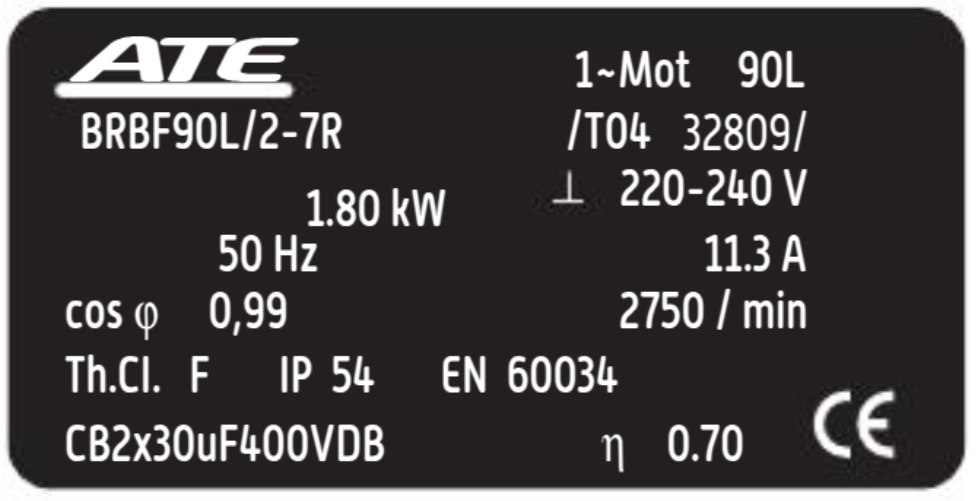
\includegraphics[width=\textwidth]{images/exo3.png}

\end{minipage}%

\vfill 

   \ding{202}\textbf{S'approprier : }

    Relever le facteur de puissance du moteur sur la plaque signalétique. \\ 
    
    \cadreblanc{10}

    \vfill 

    \ding{203} Analyser-Raisonner 

    Donnez la relation entre les grandeur $P$, $U$, $I$ et $\cos \varphi$ : 

    \cadreblanc{10}

    \vfill 

    \ding{204} Réaliser

    On a mesuré $P  = 2 360~W$,  $U=230~V$, $I=10,9~A$
    
    Calculer le facteur de puissance du moteur : 

    \cadreblanc{10}

    \vfill 

    \ding{205} Valider

    \begin{enumerate}
        \item La valeur mesurée vérifie-t-elle la valeur notée sur la plaque signalétique ? \\

    \vspace{3mm} \dotfill 

    \item La plaque signalétique indique une puissance mécanique utile $P_u = 18~kW$ et \\le rendement $\eta=0,70$ \\  
    
    Les valeurs mesurées vérifient-elles les valeurs notées sur la plaque. 

    \cadreblanc{25}
    \end{enumerate}
    
\vfill 
\end{document}